% 编辑器事项
% BUG|编辑器|LaTeX

\subsection{符号替换模式下的 bug}
按重要性排序
\begin{itemize}

\item 【完成】为什么\href{https://docs.julialang.org/en/v1/manual/unicode-input/}{这个 Julia 文档页面}中的 \lstinline|\varphi| 和 \lstinline|\phi| 粘贴到浏览器(包括符号替换规则窗口)中之后显示出来是调换的?

\item 【完成】搜索框中的 \lstinline|\phi| 和 \lstinline|\varphi| 的符号替换调换了, 但搜索的内容是正确的. 应该也按照 \lstinline|config.json| 中的规则替换(这应该和上一个 bug 有关)

\item 【完成】搜索框中不能搜索 \lstinline|\subseteq|, 因为打了 \lstinline|\subset| 以后就会直接替换成符号. 任何两个前面部分相同的命令都有这个问题

\item 【完成】自动引用公式后再连续撤销, 符号替换的紫色下划线会全部消失, 如果这时保存, tex 文件中的代码也会替换成符号

\item 【完成】有点担心符号替换会出现循环 bug, 就是修好了 A 出现 B 修好了 B 出现 C, 修好了 C 出现 A. 是否要考虑一下系统的解决方法(但愿是我多虑了).

\item 【完成】选中一段公式代码, 按 【对齐】按钮, 公式中带紫色框的符号消失

\item 【完成】删除一个带紫色框的符号再撤销, 紫色框消失

\item 【完成】代码中空心句号被替换为实心句号后, 预览中仍然是空心句号(如 “.”)

\item 【完成】使用替换功能时, 若替换的内容中的命令被替换成符号, 替换后不会出现紫色框
\end{itemize}

\subsection{Editor BUG}
按重要性排序
\begin{itemize}
\item “重新编译并发布” 按钮没有成功调用 scan 程序, 也没有显示命令行的结果(应该指定 online 路径重新运行 \verb|./PhysWikiScan .|)

\item 上传图片等待的时候提示 “PhysWikiScan 没有响应, 请稍后再试”, 过一段时间后, 图片上传成功.

\item 上传图片时如果进行其他操作会出问题(移动光标或者再次上传图片). 点击上传图片按钮后, 先在当前光标处插入代码然后再开始上传. 上传图片时在左下角显示等待的转圈动画或者进度条, 可以点 X 终止. 如果终止或其他原因上传失败, 则提示 “上传图片失败, 请手动删除图片环境”.

\item 【完成】普通用户(如 test5)使用 “下载变更文件” 按钮时出错: \verb|下载已更改文件失败:Error in api "/editor/api/download-files": findLines is not defined|

\item 预览窗口有时候会把词条显示两次(\autoref{edTODO_fig1}), 关闭后再打开可解决

\item 【完成】自动备份对 FnalNt.tex 停止了.

\item 【完成】在 “打开文件” 窗口输入 \lstinline|t.tex|, 不会出现在第一个, 是不是排序算法有问题? 其他词条也有类似的情况.

\item 【完成】自动引用一条没有 label 的公式时候只会添加 label 不会添加 \lstinline|\autoref| 命令(是否表格,图片等也有类似问题?)(在关闭符号替换模式发现的, 不确定是否和这个有关)

\item 【完成】打开词条有一定概率提示 “PhysWikiScan” 无响应

\item 【完成】已经注册的用户(如 admin)使用编辑器时不应该出现 “修改密码” 按钮

\item 【完成】自动补全设置里面的顺序不能决定候选的顺序

\item 【完成】符号替换的目标不能为 "*" (还有什么符号不能作为目标?)
\end{itemize}

\begin{figure}[ht]
\centering
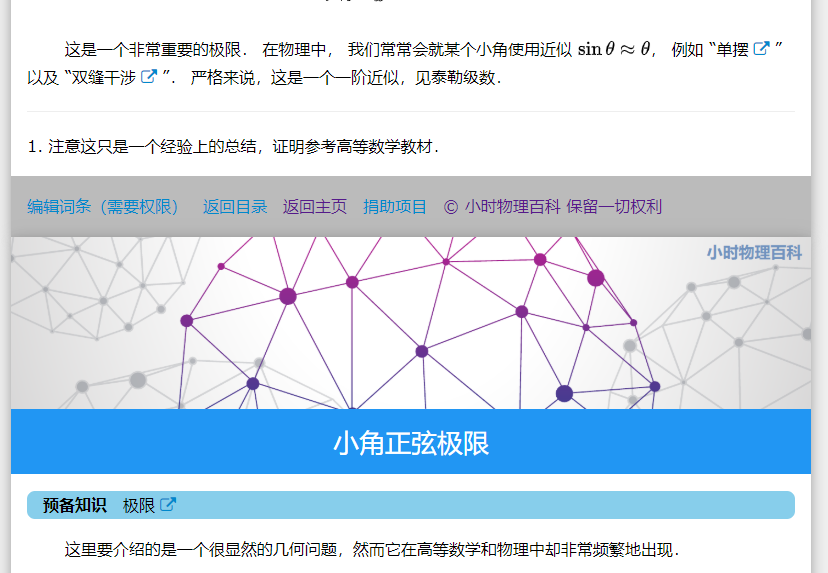
\includegraphics[width=12cm]{./figures/edTODO_1.png}
\caption{预览显示两次} \label{edTODO_fig1}
\end{figure}

\subsubsection{自动引用问题}
\begin{itemize}
\item 【完成】自动引用会弹出 “插入内部引用出错:xxxxxx” (不确定是谁的问题)
\item 【完成】自动引用(例如引用本文公式)时会出现 “PhysWikiScan 正在处理, 请稍后……” 会一直转圈.
\end{itemize}

\subsubsection{itemize 环境中的美元符号补全}
\begin{itemize}
\item 【完成】打第一个美元符号不会出现一对美元符号 $abc^2$

\item 【完成】手动打第二个美元符号时会出现两个 $1 + x (x \in X)$
\end{itemize}

\subsubsection{表格以后的正文高亮}
【完成】 “原子单位\upref{AU}” 的表格中和表格结束以后所有字体都变成了橙色

\subsection{Editor TODO}

\begin{itemize}
\item 定义,定理,itemize 等环境中(不包括 equation) 的普通文字不需要变绿

\item 在编辑百科时, 禁止关闭 “自动替换空心句号为实心” 功能(把开关锁定)

\item 删除词条时同时删除 \verb|changed/| 和 \verb|online/| 目录中对应的 html 和图片文件 (图片名格式为 \verb|词条名_编号.拓展名|)

\item 保存按钮的 tip 改为 \verb|保存并编译(Ctrl+S)|

\item 【完成】插入 \verb|\autoref{}| 的时候在后面多加一个空格(前面不需要).

\item 增加一个注释按钮, 图标为 \verb|%|, 下拉菜单有两个按钮, 一个是 “注释选中内容”(默认), 另一个 “取消注释选中内容”. 注释时, 每个插入的 \verb|%| 后面需要再插入一个空格. 如果选中的内容不是从行首开始, 那么在选中内容之前加上 \verb|%| 和空格. 如果选中内容的最后不是一整行, 那么注释以后在选中内容后面换一行. 总之确保有且仅有被选中内容被注释. 注意考虑只选中一行中某部分的情况. 取消注释时, 删除选中内容中行首的 \verb|%| 以及后面的空格(如果有). 如果选中内容第一个字符是 \verb|%| (无论是不是行首), 也将它和后面的空格(如果有)删掉.

\item 【完成】code 按钮支持新语言: python, pythonC(python 命令行), julia, markdown, bash, makefile, json, git, cmake, regex, latex

\item 【完成】符号替换设置打开时, json 编辑窗自动排版格式太慢, 是否考虑关闭时自动排版并保存排版后的文件?

\item 【完成】在编辑器加载页面(有转圈动画的那个)用小字显示 “建议使用 Chrome 或 Chromium 内核的浏览器”

\item 【完成】替换模式下上传图片后不需要再提示 “该图片已存在, 是否替换?”

\item 上传图片的时候允许额外上传一个其他格式的文件(例如源码文件), 重命名为和图片文件相同.

\item 【完成】历史版本列表中应该显示所有用户的备份以及用户名, 目前好像仅显示当前用户的, 在 i 图标后面的文字改为 \verb|请选择要恢复的版本(使用北京时间)|, “search backup name”  改为 “搜索”

\item 创建词条的窗口在文件名下方添加一个选填栏 “关键词”,在上方的说明改为 \lstinline+请输入标题(如“角动量守恒”),文件名(如"AngMom")和关键词.文件名不能超过 6 个字符,只能含有字母或数字,不能以数字开头; 关键词格式如 “关键词1|关键词2|关键词3”, 建议填写以方便检索.+

\item 创建词条后, 在文件第二行注释关键词, 如 \lstinline+% 关键词1|关键词2|关键词3+, 光标停留在第四行. 如果创建时没有填写关键词, 则第二行为空, 光标停在第三行

\item 删除一个文件时, 图片和源文件也要一并删除(包括 figures 中所有格式为 \verb|词条名_数字.任意拓展名| 的文件, online, changed 中对应的 svg 和 png 文件.

\item 每五分钟的备份也要包括图片和源文件(即 figures 文件夹中所有格式为 \verb|词条名_数字.任意拓展名| 的文件), 命名规则和 tex 文档一样. 只有图片文件内容被改变时才备份(可以通过 hash 判断或者逐字节对比).

\item 【先不要做】考虑用 Electron 做一个离线版的 wuli.wiki/note. 不需要网络连接(但 mathtype 应该需要网络才能用), 功能完全一样, 除了: 添加一个按钮可以设置用户名, 如果没有用户名, 则弹出提示框输入用户名 “请输入任意用户名, 以后可以在菜单栏修改”. 不需要任何密码. 另外增加一个按钮设置输入输出路径, 相当于 \verb|littleshi.cn/root/user/|. 默认路径为 \verb|Desktop/wuli.wiki-note/|

\item 【完成】预览窗口中的 css 使用 PhysWikiScan 输出文件夹中的 css (不同用户可能不一样)

\item 【完成】“重新编译所有内容及目录树” 按钮的输出框不能全选复制, 增加一个 “复制” 按钮.

\item 【完成】“重新编译所有内容及目录树” 按钮右边加一个类似公式的下拉选项, 可以选择 “编译并发布” 或者 “编译但不发布”. 前者输出到 online 文件夹, 后者输出到 changed 文件夹

\item 【完成】在管理员和用户笔记的界面中添加 “重新编译所有内容及目录树” 按钮, 按下后调用 \lstinline|PhysWikiScan . --path...|  命令.

\item 【完成】删除 main.tex 时提示 “该文件不能被删除”

\item 【完成】禁止创建文件名为 \lstinline|index.tex| 的文件

\item 【完成】打开词条页面的 “i” 图标和后面的提示可以删掉, 然后把搜索框里面的英文改成 “搜索标题或文件名……”

\item 【完成】设置菜单中 “恢复默认设置” 时, 恢复到 note-template 中的设置

\item 【完成】增加一个脚注按钮, 插入 \lstinline|\footnote{脚注}|, 并自动选中 “脚注”

\item 【完成】增加一个代码按钮, 图标为 \lstinline|</>|, 按下以后弹出输入框 “请指定语言(不指定则没有高亮)” \lstinline|"\\begin{lstlisting}[language=输入的语言]\n${1}\n\\end{lstlisting}"|

\item 【完成】“插入词条引用按钮” 同时也插入词条的中文名, 且自动选中中文名以便修改. 例如 “词条示例\upref{Sample}”

\item 【完成】保存缓慢时区分是因为网络缓慢还是 PhysWikiScan 无响应. 如果是前者, 就一直尝试连接直到手动关闭提示框.

\item 【完成】上传的图片保存文件名的格式为 \verb|词条名_序号.后缀名|

\item iOS 的 Safari 中拖动文字导致拖动整个屏幕(只有从论坛登录才会,不是编辑器本身的问题)

\item iOS 的 Safari 中选中文字光标位置错误

\item iOS 的 Safari 中键盘有时候无法弹出(即使外接键盘)

\item 【完成】选中一段文字后点击链接按钮, 插入 \lstinline|\href{http://www.example.com}{被选中的文字}|, 自动选中网址
\end{itemize}

\subsubsection{公式编辑器相关}
\begin{itemize}
\item 已使用 \href{http://www.wiris.net/client/editor/resources/help.html?v=7.9.0.6564}{MathType Web} 作为公式编辑器插件(比上面那个 codecogs 颜值高多了).初次使用该功能时将动态加载插件,国内测试加载时间约为 10-12s,此后使用可直接打开无需再加载.
目前公式编辑器仅在 Chrome 上测试正常,其他平台未知.已知的 bug 如下:

\item 由于站点问题,编辑器加载有时会失败(提示 Connection Reset),需要支持自动重新加载

\item 因为是基于 CSS 排版且用的不是数学专用字体(Times New Roman),编辑中的公式显示会和 MathJax 显示的存在样式和位置上的出入(TODO:字体看看有没有办法引用 MathJax 的字体)

\item Edge 下点击 “确定” 按钮不能正常插入公式

\item 移动端下不能显示 “确定” 和 “取消” 按钮

\item TODO:对公式编辑器支持插入的符号进行完善,已经按照百科词条加了一些常用符号,看还有什么需求(是否需要一个复制 LaTeX 而不关闭编辑器的按钮?)

\item TODO:编辑器的布局改进,显示位置调整,等等

\item GUI 公式编辑器插入公式

\item 【暂时不需要】TODO:因该插件不支持 physics 宏包,选中大多数词条中现有公式的 LaTeX 打开编辑器,是无法正确显示的(如 $I = \int\bvec j \vdot \dd{\bvec S}$ 选中这段打开编辑器),并且由编辑器生成的 LaTeX 也不符合百科的命令规范(但显示效果基本一致),需编写 processor 对命令进一步转换,如将$\frac{\partial^{n}{\cdot}}{\partial{\cdot}^{n}}$ 转换成 $\pdv[n]{\cdot}{\cdot}$,$\left\langle{\cdot}\vert{\cdot}\right\rangle$ 转换成 $\braket{\cdot}{\cdot}$ etc.
\end{itemize}

\subsection{PhysWikiScan BUG}

\subsection{changed}
\begin{itemize}
\item 【完成】changed.txt 中只有一个词条的时候, 发布词条会提示错误. 为空时也会错误?
\end{itemize}

\subsubsection{表格标签多次定义}
【完成】删除某个表格再重新插入一个具有同样标签的表格就会出现 “标签多次定义” 的错误.

\subsubsection{表格标题}
【完成】第二个表格会具有第一个表格的标题

\subsection{PhysWikiScan TODO}
\begin{itemize}
\item 深度兼容 \lstinline|\(\)|, 和 \lstinline|$$| 完全一样对待

\item 在每个词条底部加上目录树的链接
\end{itemize}

\subsubsection{改用 MathJax2}
【完成】MathJax3 在 iOS 的 Safari 上显示有时候公式上半部分消失. 注意当前的 MathJax3 文件夹复制一个备份

\subsubsection{不要使用 MathJax 的 newcommand}
\begin{itemize}
\item 【完成】而是直接进行命令替换, 从而增加公式代码在其他网站的兼容性
\end{itemize}

\subsubsection{脚注加上返回链接}
参考维基百科和知乎. 或者是否可以做成点了以后直接弹出一个子窗口而不是跳到底部? 如何实现?
